\documentclass{article}\usepackage[]{graphicx}\usepackage[]{color}
%% maxwidth is the original width if it is less than linewidth
%% otherwise use linewidth (to make sure the graphics do not exceed the margin)
\makeatletter
\def\maxwidth{ %
  \ifdim\Gin@nat@width>\linewidth
    \linewidth
  \else
    \Gin@nat@width
  \fi
}
\makeatother

\definecolor{fgcolor}{rgb}{0.345, 0.345, 0.345}
\newcommand{\hlnum}[1]{\textcolor[rgb]{0.686,0.059,0.569}{#1}}%
\newcommand{\hlstr}[1]{\textcolor[rgb]{0.192,0.494,0.8}{#1}}%
\newcommand{\hlcom}[1]{\textcolor[rgb]{0.678,0.584,0.686}{\textit{#1}}}%
\newcommand{\hlopt}[1]{\textcolor[rgb]{0,0,0}{#1}}%
\newcommand{\hlstd}[1]{\textcolor[rgb]{0.345,0.345,0.345}{#1}}%
\newcommand{\hlkwa}[1]{\textcolor[rgb]{0.161,0.373,0.58}{\textbf{#1}}}%
\newcommand{\hlkwb}[1]{\textcolor[rgb]{0.69,0.353,0.396}{#1}}%
\newcommand{\hlkwc}[1]{\textcolor[rgb]{0.333,0.667,0.333}{#1}}%
\newcommand{\hlkwd}[1]{\textcolor[rgb]{0.737,0.353,0.396}{\textbf{#1}}}%
\let\hlipl\hlkwb

\usepackage{framed}
\makeatletter
\newenvironment{kframe}{%
 \def\at@end@of@kframe{}%
 \ifinner\ifhmode%
  \def\at@end@of@kframe{\end{minipage}}%
  \begin{minipage}{\columnwidth}%
 \fi\fi%
 \def\FrameCommand##1{\hskip\@totalleftmargin \hskip-\fboxsep
 \colorbox{shadecolor}{##1}\hskip-\fboxsep
     % There is no \\@totalrightmargin, so:
     \hskip-\linewidth \hskip-\@totalleftmargin \hskip\columnwidth}%
 \MakeFramed {\advance\hsize-\width
   \@totalleftmargin\z@ \linewidth\hsize
   \@setminipage}}%
 {\par\unskip\endMakeFramed%
 \at@end@of@kframe}
\makeatother

\definecolor{shadecolor}{rgb}{.97, .97, .97}
\definecolor{messagecolor}{rgb}{0, 0, 0}
\definecolor{warningcolor}{rgb}{1, 0, 1}
\definecolor{errorcolor}{rgb}{1, 0, 0}
\newenvironment{knitrout}{}{} % an empty environment to be redefined in TeX

\usepackage{alltt}
\usepackage{authblk}  % To create author affiliations
\usepackage[round]{natbib}
\usepackage{graphicx}


\title{Lab Report Title}

\author[1]{First Author}
\author[2]{Second Author}
\author[1]{Third Author}
\author[3]{Fourth Author}
\affil[1]{Pitzer College, address...}
\affil[2]{Scripps Collge, address...}
\affil[3]{Pomona College, address...}

%\date{} % Remove Comment if you want to remove the date
\IfFileExists{upquote.sty}{\usepackage{upquote}}{}
\begin{document}

\maketitle

\begin{abstract}
This is my abstract for a minimum working Rnw for creating a lab report...

\end{abstract}

\section{Introduction}


\section{Methods}

\subsection{Site Description}

Add if appropriate .. e.g. where you did your research if no in the lab... \citep{dris2015beyond}

\subsection{Procedures}

\subsection{Statistical Analysis}

\section{Results}

Some cool image...that are already made...(Figure~\ref{fig:boxplot}).

\begin{figure}
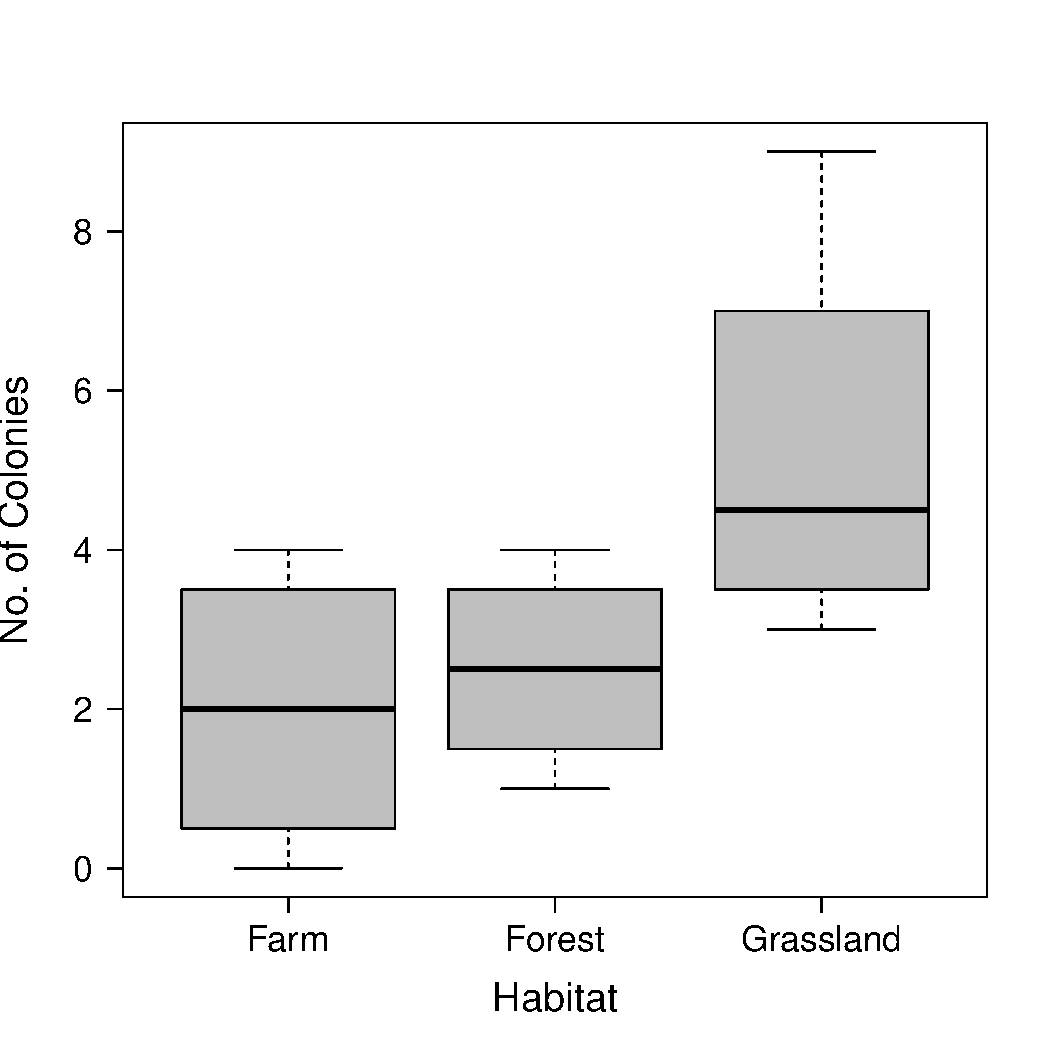
\includegraphics[width=\textwidth]{figure/boxplot-1} % This can be a pdf, jpg, or png file
\caption{This is a boxplot.}
\label{fig:boxplot}
\end{figure}

Or you can make figure using R... (Figure~\ref{fig:carsplot}).

\begin{figure}
\begin{knitrout}
\definecolor{shadecolor}{rgb}{0.969, 0.969, 0.969}\color{fgcolor}\begin{kframe}
\begin{alltt}
\hlkwd{plot}\hlstd{(cars)}
\end{alltt}
\end{kframe}
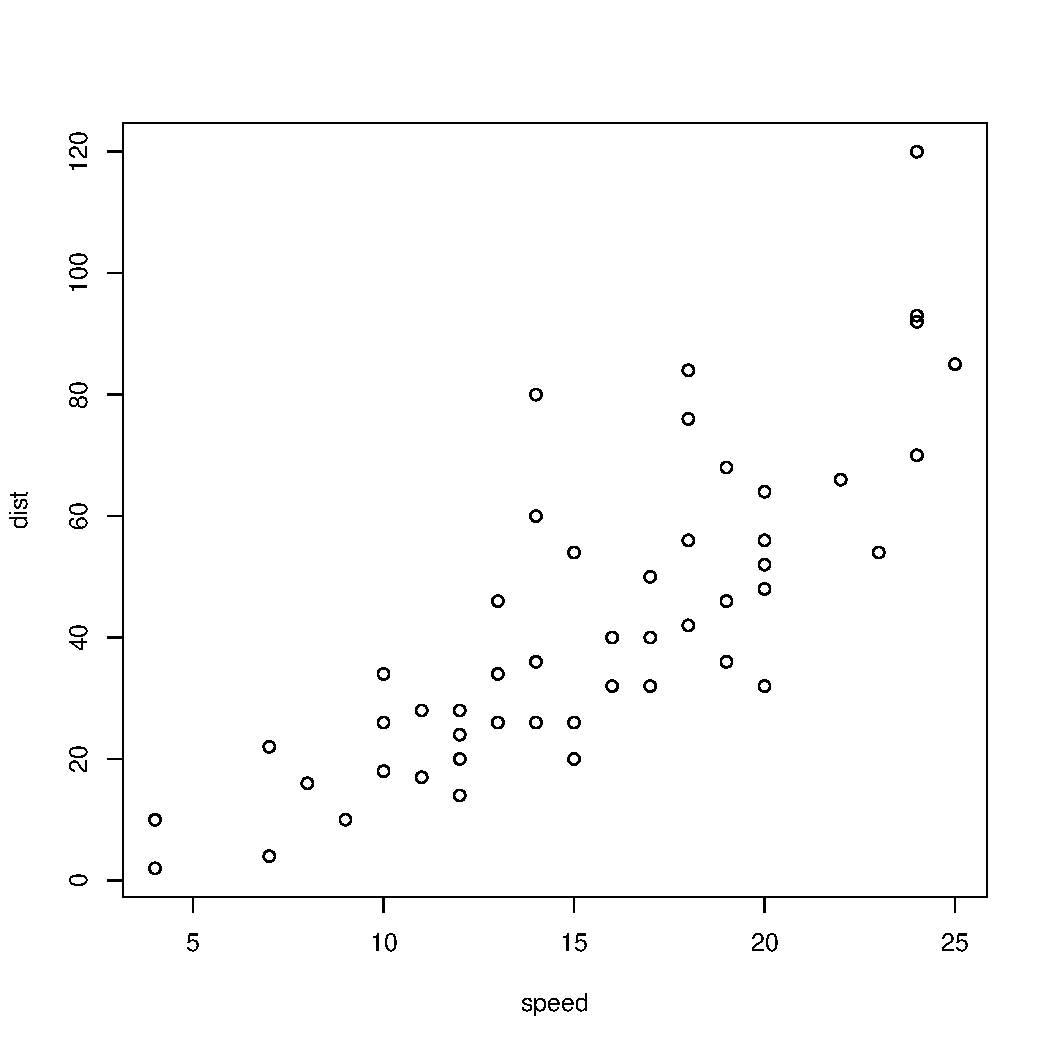
\includegraphics[width=\maxwidth]{figure/unnamed-chunk-1-1} 

\end{knitrout}
\caption{A figure that can be made using R and we can make the r code disappear too...}
\label{fig:carsplot}
\end{figure}

\section{Discussion}

\section{Conclusion}

\bibliographystyle{cbe} % To get this to work, we need the cbe.bst file in the directory that you are using to run the rnw file!

\bibliography{bibexample}



\end{document}
